\documentclass[11pt]{amsart}
\usepackage[centering]{geometry} % See geometry.pdf to learn the layout options. \tauhere are lots.
\geometry{letterpaper} % ... or a4paper or a5paper or ...
%\geometry{landscape} % Activate for for rotated page geometry
%\usepackage[parfill]{parskip} % Activate to begin paragraphs with an empty line rather than an indent
\usepackage{hyperref}
\usepackage{graphicx}
\usepackage{mathrsfs}
\linespread{1.3}
\usepackage{amssymb}
\usepackage{epstopdf}
\usepackage{amscd}
\usepackage{comment}
\usepackage[english]{babel}
\usepackage{tikz}
\usepackage{latexsym}
\usepackage{float}
\usetikzlibrary{calc}
\usetikzlibrary{shapes.arrows}
\usetikzlibrary{shapes.geometric}
\renewcommand{\thesection}{\Roman{section}} 

\newtheorem{theore}{\tauheorem}
\newtheorem{propositio}{Proposition}
\newtheorem{theorem}{\tauheorem}[section]
\newtheorem{thm}{Main \tauheorem}[section]
\newtheorem{theor}{\tauheorem}[section]
\newtheorem{conj}{Conjecture}
\newtheorem{cor}[thm]{Corollary}
\newtheorem*{mthm}{Main \tauheorem}
\newtheorem{proposition}[theorem]{Proposition}
\newtheorem{corollary}[theorem]{Corollary}
\newtheorem{claim}[theorem]{Claim}
\newtheorem{lemma}[theorem]{Lemma}
\newtheorem{remark}[theorem]{Remark}
\newtheorem{example}[theorem]{Example}
\newtheorem{definition}[theorem]{Definition}
\newtheorem{question}[theorem]{Question}
\newtheorem{conjecture}[theorem]{Conjecture}
\newtheorem{summary}[theorem]{Summary}
\newtheorem{fact}[theorem]{Fact}
\newtheorem*{theorem-non}{\tauheorem}
\newtheorem*{lemmam}{Lemma}
\newtheorem*{remarkm}{Remark}
\newtheorem*{factt}{Fact}
\newtheorem*{quest}{Questions}

\DeclareMathOperator{\Spec}{Spec}
\DeclareMathOperator{\Hom}{Hom}
\DeclareMathOperator{\cha}{char}
\DeclareMathOperator{\Sym}{Sym}
\DeclareMathOperator{\norm}{norm}
\DeclareMathOperator{\Proj}{Proj}
\DeclareMathOperator{\Bl}{Bl}
\DeclareMathOperator{\Pic}{Pic}
\DeclareMathOperator{\codim}{codim}
\DeclareMathOperator{\Ker}{Ker}
\DeclareMathOperator{\\tauors}{\tauors}
\DeclareMathOperator{\Supp}{Supp}
\DeclareMathOperator{\red}{red}
\DeclareMathOperator{\rk}{rank}
\DeclareMathOperator{\Amp}{Amp}
\DeclareMathOperator{\ord}{ord}
\DeclareMathOperator{\Jac}{Jac}
\DeclareMathOperator{\gal}{Gal}
\DeclareMathOperator{\GL}{GL}
\DeclareMathOperator{\psl}{PSL}
\DeclareMathOperator{\Aut}{Aut}
\DeclareMathOperator{\SL}{SL}
\DeclareMathOperator{\End}{End}
\DeclareMathOperator{\tr}{tr}
\DeclareMathOperator{\Aff}{Aff}
\DeclareMathOperator{\Stab}{Stab}


\author{Etale Inc.}
%\address{\tiny{Federico Buonerba\newline Courant Institute of Mathematical Sciences,
% New York University, 
% 251 Mercer Street, 
% New York, NY 10012\newline
% Etale Inc, WeWork 300 Park Ave, New York, NY 10022}}
% \email{federico.buonerba@etale.com}

%\author{Matthew Cushman} 
%\address {\tiny{Matthew Cushman \newline Etale Inc,WeWork 300 Park Ave, New York, NY 10022}}
%\email{matt.cushman@etale.com}

 
 
\DeclareGraphicsRule{.tif}{png}{.png}{`convert #1 `dirname #1`/`basename #1 .tif`.png}
\title{Modeling risk in the cryptocurrency universe}
%\date{} % Activate to display a given date or no date
\begin{document}
\begin{abstract}
 We describe a linear model that explains correlation among historical log-returns of
 Bitcoin-denominated cryptocurrency prices. 



\end{abstract}
\maketitle
\section{Introduction}
The goal of our work is present the first attempt to understand covariance among cryptoassets.
Since the legendary intuition of Markowitz, estimating correlations among any assets has been a
central topic of research and interest for all those involved in financial markets, being the
first and most important step in constructing a well-balanced portfolio. As it happens
quite often in science, naive estimations tend to lead to surprisingly bad results, and the source
of failure is in general hard to understand. In the specific case of assets returns, assume we 
wish to understand volatility among assets $A_1,\cdots , A_n$. For each $i=1,\cdots , n$ we are provided with a
time-series $r_{i,1},\cdots , r_{i,\tau}$ of historical returns, sampled periodically over $\tau$ periods of time.
In this case, one would consider a matrix $R=(r_{i,t})$ and attempt to naively estimate covariances
by simply computing $C=R^T\cdot R$, or an adjusted variand thereof to deal with outstanding means.
Upon some further reflection, interpreting $C$ as the correct covariance matrix turns out to be a poor idea:
the size of $C$ is such that this matrix is going to be poorly conditioned. For example if $n>\tau$ 
the matrix itself will not be invertible, and therefore lead to portfolios that are apparently riskless.
Moreover, even in the good quality data scenario $\tau=n$, correlation is not stationary as the market structure
changes over time.
In this type of situations, one is led to think that an intermediate step in between estimating 
the covariance matrix $C$, and blindly interpreting it, is to somehow organize a dimensionality
reduction: form a hierarchical 
structure of clusters as dictated by the structure of $C$, and then interpret correlations using
the hierarchy. This line of thought has many advantages, ranging from robustness to interpretability.
We will implement this idea by fitting a multi-factor linear model.
This means that we approximate asset returns
using a linear subspace $S$ of dimension $d<<n$. 
The poorly conditioned nature of $C$ suggests that there exists $d<<n$ 
such that virtually all the variance of asset returns can be explained via $S$.
One simple-minded technique to achieve this goal is to use principal component analysis (PCA), which simply
means to define $S$ as the span of the $d$ eigenvectors of $C$ whose eigenvalues are highest. This method, albeit 
gaining in robustness, might still lack an adequate amount of interpretability - $S$ looks very
artificial.
We finally arrive to the notion of multi-factor model. Instead of blindly picking $S$ as the result of
PCA, we add our key intuition of the real world. We know that there are some
simple factors that are naturally significant sources of risk, 
and whose value should naturally cluster assets returns together. For example, the size or total value
of an asset may be such factor; the frequency of trades may be another factor.
An important technical condition that every factor should satisfy is: it should depend on quantities that change very slowly in
time. For this reason one tends to pick factors that can be estimated as averages/max/min over long periods of time.
Assume for each asset $i$ and time $t$, we have an estimate of $d$ factors, {\it i.e.} 
$X_{1,i,t},\cdots , X_{d,i,t}$. A multi-factor model is then obtained by regressing retruns against factors:
\begin{equation}
r_{i,t}= \sum_{k=1}^d \beta_{t,k} X_{k,i,t} + \epsilon_{i,t}
\end{equation}
where the intercept is taken into account by assuming $X_{d,i,t}=1$ for every $i,t$.
The slow-varying nature of factors in time leads to our crucial estimate:
\begin{equation}
R^T\cdot R \sim X^T(\beta_{\tau}^T\cdot \beta_{\tau})X + \text{diag}(\epsilon^2)
\end{equation}
This approach has many visible advantages:
\begin{itemize}
\item Enhanced stability, since eigenvalues of the right-hand-side are no smaller than the entries of 
$\text{diag}(\epsilon^2)$.
\item Robustness against outliers and missing data points.
\item Simple and intuitive understanding of individual factor loadings $\beta_{t,k}$.
\item Flexibility of the model, in that different combinations of factors can be tested,
which allows to view asset returns from different angles.
\end{itemize}
The discussion above applies to any family of assets. From now on, we focus specifically
on the universe of cryptoassets. For our experiments we decided to select few very simple
and intuitive factors that have been widely used in financial modeling, leaving aside more
exotic ones that may be relevant to the crypto world - factors such as price of electricity,
number of miners on the blockchain, amount of activity on GitHub, sentiment analysis of
Twitter data, and so on.

\section{Our model}
We can now dive into more technical details about our model. We consider a universe of
$33$ coins, that have been selected according to three criteria:
\begin{enumerate}
\item High market cap
\item Availability of historical market data
\item Not being a stablecoin (as the purpose of stablecoins is to eliminate volatility relative to a benchmark)
\end{enumerate}

For each such coin we look exclusively at transactions to BTC:
exchange rates are with respect to BTC, volumes are volumes of coins traded with BTC over all exchanges.
Coins we will consider are:\newline
'BTC' 'ETH' 'XRP' 'BCH' 'EOS' 'XLM' 'LTC' 'ADA' 'XMR' 'IOTA' 'TRX' 'ETC'
 'DASH' 'NEO' 'XEM' 'BNB' 'ZEC' 'OMG' 'LSK' 'ZRX' 'QTUM' 'DOGE' 'BTS'
 'DGB' 'ICX' 'STEEM' 'AE' 'WAVES' 'SC' 'REP' 'PPT' 'GNT' 'STRAT'\newline
Let $c$ denote any of the about coins and $T^*=[T_0,T_1]$ a time interval of $T$ days.
Let $P_c=(p_{c,1},...,p_{c,T})$ denote the vector of daily exchange rates for coin $c$ with respect to BTC 
over period $T^*$.
Likewise let $R_c=(r_{c,1},...,r_{c_T})$ denote the vector of daily returns, $S_c=(s_{c,1},...,s_{c,T})$
the vector of daily number of coins outstanding, and $V_c=(v_{c,1}, ..., v_{c,T})$ the vector of daily traded
volumes in BTC.
Our risk factors are:

%% mwc comment:  we should name the factors.  would also be good to try some variants on them (we probably shouldn't document every tweak as we want something propritary as well perhaps).  We should also include a historical plot of cumulative returns to the factors

\begin{itemize}
\item Standard deviation of returns std$(R)$.
\item Strength of returns $$\sum_{t=1}^n \log(1+r_{c,t})$$
\item High-low of rates $$\log(\frac{\max_t p_{c,t}}{\min_t p_{c,t}})$$
\item Average log market cap $$\frac{\sum_{t=1}^T\log(p_{c,t}\times s_{c,t})}{T}$$
\item Volume turnover $$\frac{\sum_{t=1}^T v_{c,t}}{(\frac{\sum_{t=1}^T s_{c,t}}{T})}$$
\end{itemize}
Denote by $X_{k,c,t}$ the value of factor $k$ at time $t$ for coin $c$. Our model estimates returns
as a linear combination:
\begin{equation}
r_{c,t}= \sum_{k=1}^5 \beta_{t,k} X_{k,c,t} + \epsilon_{c,t}
\end{equation}
Where factor loadings $\beta_{t,k}$ are obtained through weighted linear regression, and $\epsilon_{c,t}$
is an unpredictable error term. Observe that regressing using the method of ordinary least squares assumes
implicitly that $\epsilon_{c,t}$ are independent and identically distributed. 
In particular, this method assumes that the variance of time-series $(\epsilon_{c,t})_{t\in T^*}$,
estimated as $\text{var}((\epsilon_{c,t})_{t\in T^*})\sim \text{var}((R_{c}))$, is independent of the coin $c$.
This independence of variance is not detected here, i.e. we are in presence of heteroskedasticity.
In such situation it is more appropriate to use the method of weighted least squares, which is an ordinary
least squares regression using time-series $\frac{R_c}{\text{std}(R_{c})}$ and 
$\frac{(X_{k,c,t})_{t\in T^*}}{\text{std}(R_{c})}$. The reason for this is that 
dividing by $\text{std}(R_{c})$ normalizes the error terms to have the same variance. Summing up, our error
terms and factor loadings are estimated through the following ordinary least squares problem:
\begin{equation}
\frac{r_{c,t}}{\text{std}(R_{c})}= \sum_{k=1}^5 \beta_{t,k} \frac{X_{k,c,t}}{\text{std}(R_{c})} + \epsilon_{c,t}
\end{equation}
The reader may observe that our definition of factors are slightly 
different from those commonly encountered in the literature.
In particular,the following factors have been changed:
first, we look at log market cap averaged over $T^*$, rather than log market cap at time $T$;
second, we look at volume turnover, not turnover, the difference being that in our numerator we
do not have number of coins traded, but the amount of coins traded expressed in BTC - in particular,
the exchange rate between our coin and BTC is embedded in volume turnover.
The reason for this slight difference is two-fold. First, factors computed using time-wise averages
tend to vary much less over time. Second, our linear model performed better when implemented with
these definitions than with classical ones.\newline
In detail, we considered 140 time intervals, of the form 
$[T_0,T_1], [T_0+1\text{day}, T_1+1\text{day}],..., [T_0 + 139\text{days}, T_1+139\text{days}]$
with $T_0=$January 07 2018, and $T_1=$April 01 2018.
The model utilizing our definitions beat the model utilizing classical definitions by 89-51,
where the comparison is by way of $R^2$ score of linear regressions. 
The linear model with our definition obtains, in the above-mentioned time intervals, a
huge spectrum of $R^2$ scores averaging $24\%$.
The following scatter plot shows the time-series of $R^2$ scores across these 140 days.
\begin{figure}[H]
  \caption{R2 scores}
  \centering
    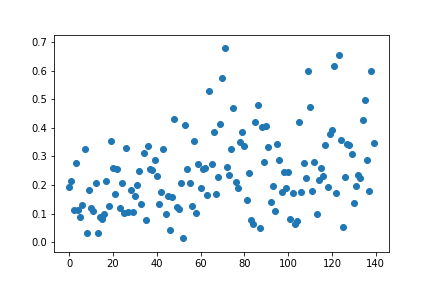
\includegraphics[scale=0.3]{r2_scatter.png}
\end{figure}
The next plot shows the time-series of cumulative factor returns obtained by our model, in the same period of time.
\begin{figure}[H]
  \caption{Cumulative factor returns}
  \centering
    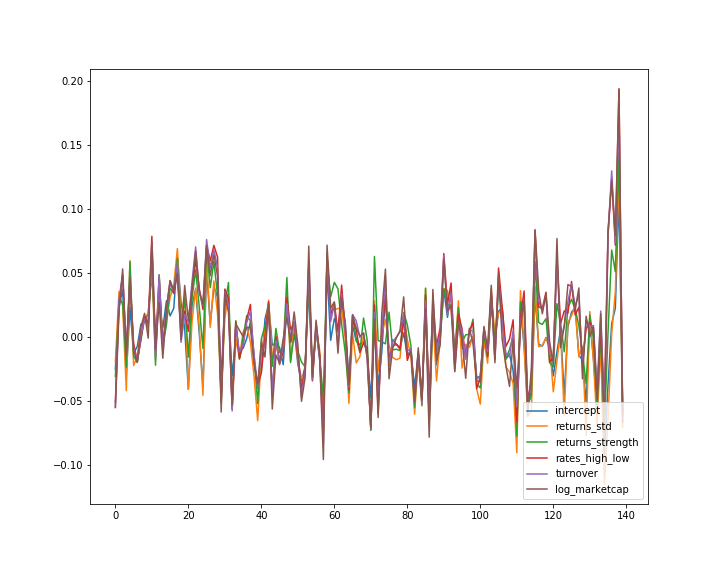
\includegraphics[scale=0.4]{factor_returns.png}
\end{figure}
Here the term intercept is simply the constant term of our regression.\newline 
The following heatmaps represent correlations between coin returns computed
in the last time interval, namely May 26 2018 to August 18 2018. The first heatmap shows raw correlations, while
the second shows those computed by our model.
\begin{figure}[H]
  \caption{Raw correlations}
  \centering
    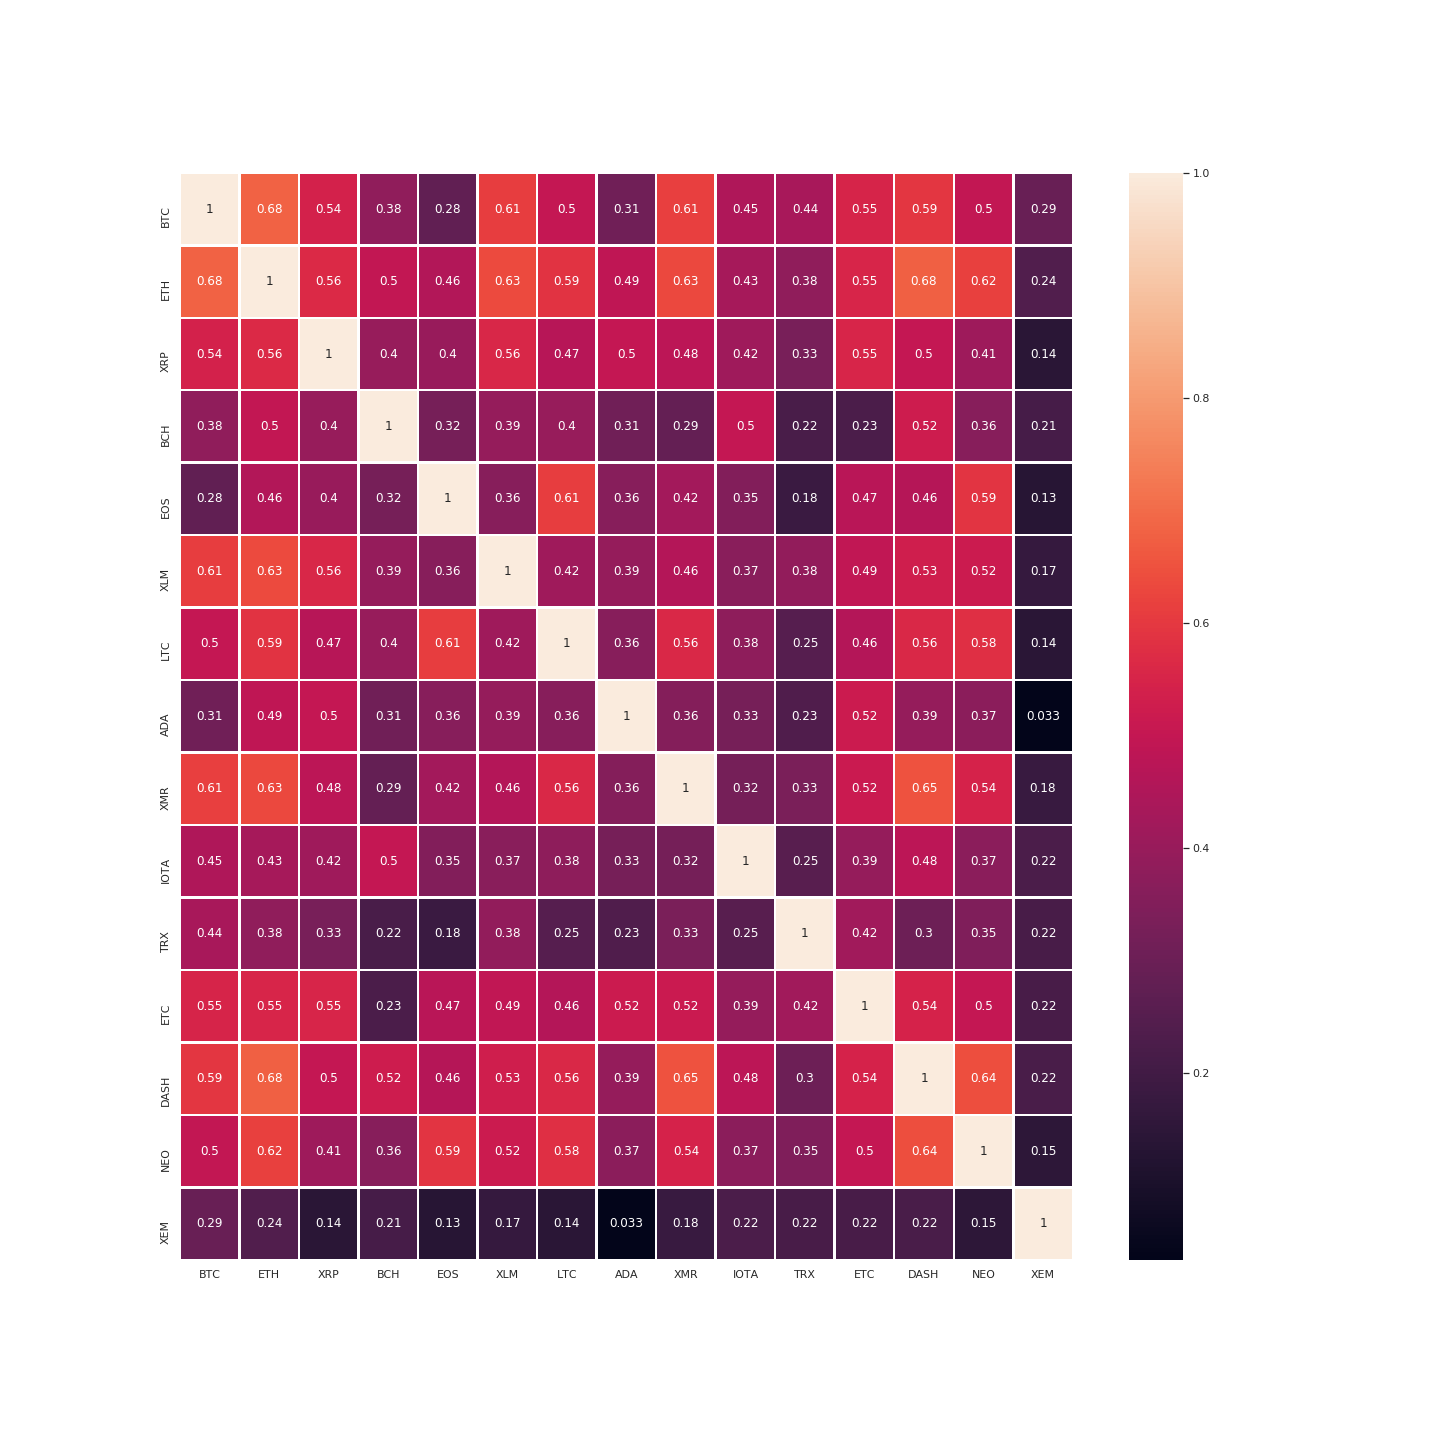
\includegraphics[scale=0.3]{raw_corr.png}
\end{figure}
\begin{figure}[H]
  \caption{Model correlations}
  %\centering
    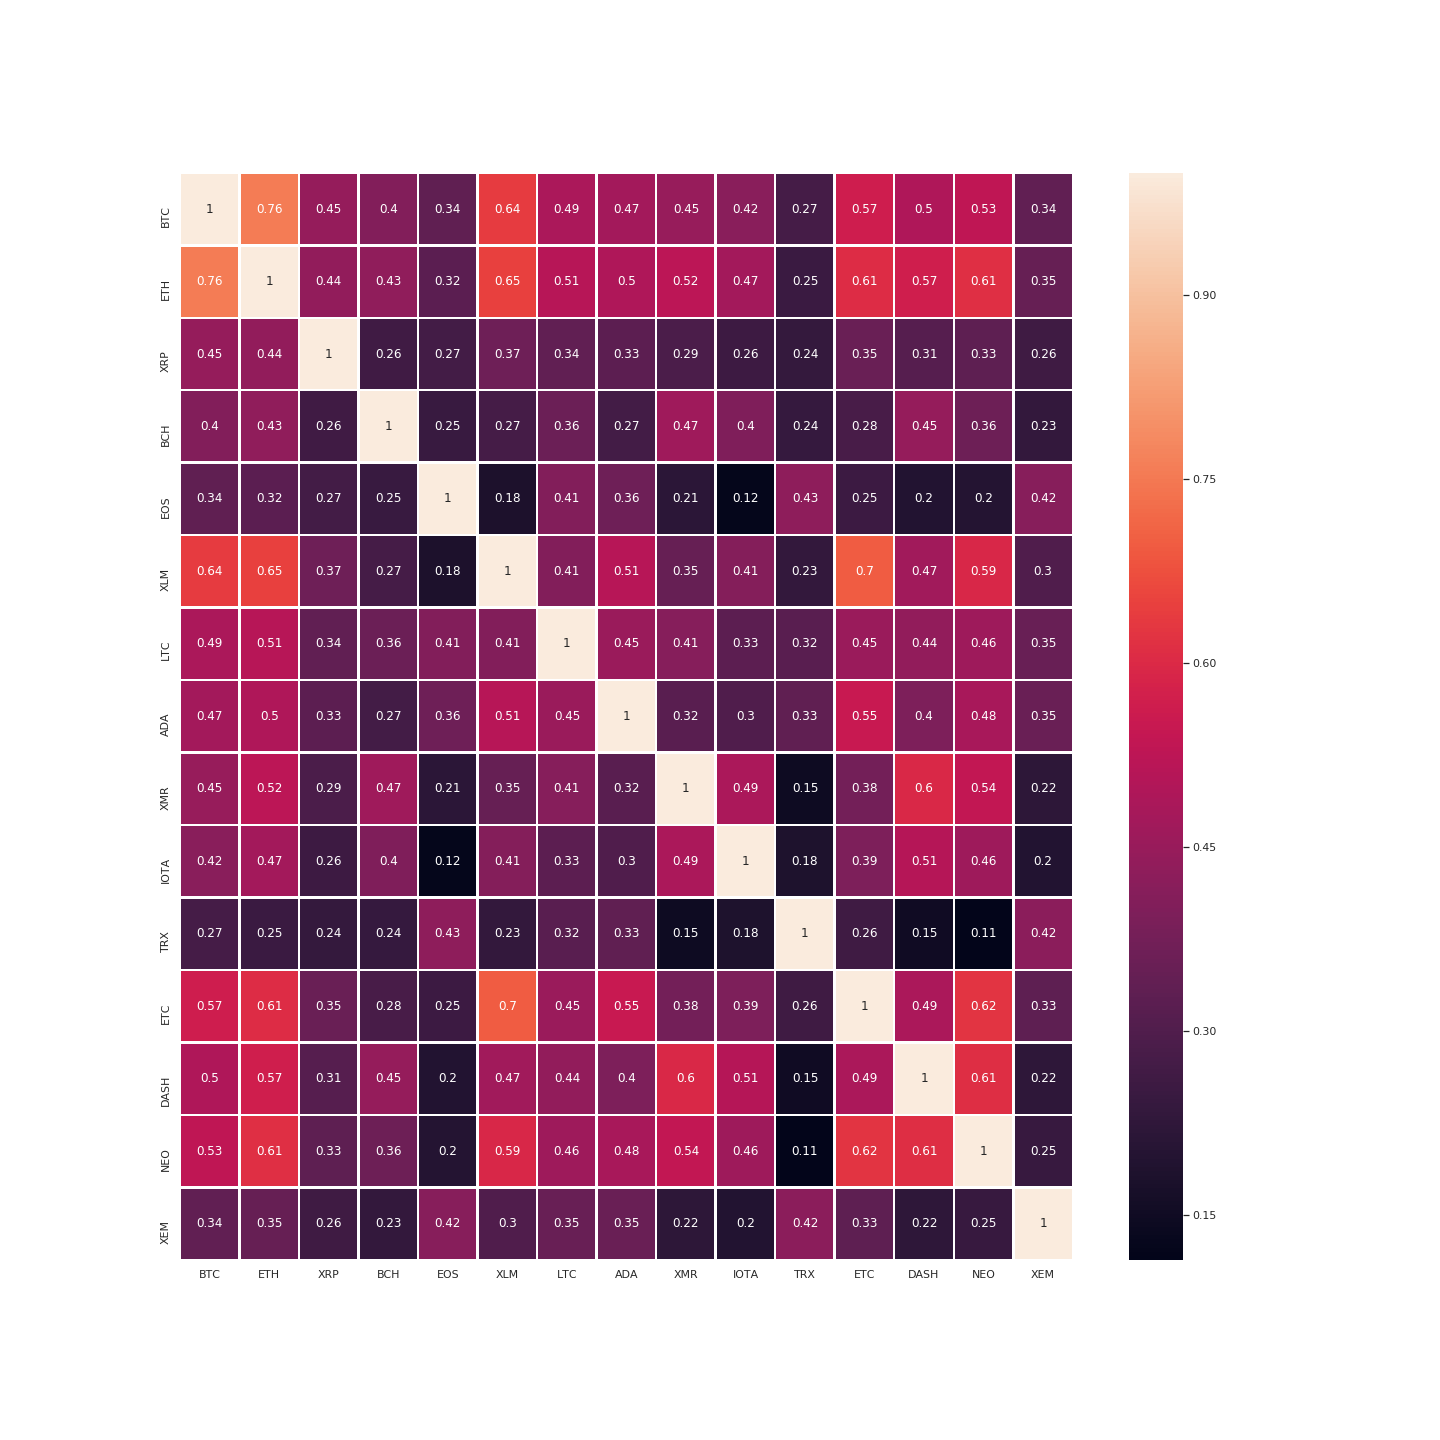
\includegraphics[scale=0.3]{model_corr.png}
\end{figure}


\section{Portfolio hedging}
We can describe a first application of our method, namely construction of optimal portfolios.
The methodology goes back to Markowitz. Given a time $T$, a collection
of coins $C$, we assume a vector of estimated coin returns, at time $T$, is given and denoted $\alpha=(\alpha_c)_{c\in C}$.
Moreover, let $\Sigma$ denote the covariance matrix for historical coin returns up to time $T$.
Our goal is to invest a unit amount of capital minimizing risk and for a given value of expected return $\mu$. 
We wish to find a vector of weights $w=(w_c)_{c\in C}$ solving the following quadratic optimization problem:\newline
\textit{Minimize $w\cdot \Sigma\cdot w^T$ under constraints $\sum_c w_c=1$ and $\sum_c \alpha_cw_c=\mu$}.\newline
This problem is easily solved via Lagrange multipliers, and it is equivalent to:\newline
\textit{Minimize $w\cdot \Sigma\cdot w^T -\lambda \alpha\cdot w$ under constraint $\sum_c w_c=1$}.\newline
The relation between $\lambda$ and $\mu$ in the above formulations can be easily computed.
As an example, say we expect ETH to enjoy a superior return on August 18 2018, i.e. $\alpha=(1,0,...,0)$.
We would like to hedge our portfolio under this expectation.
Setting $\lambda=1$ and using correlations estimated between May 26 2018 to August 18 2018,
we get the following array of weights $w$ - where a negative weight suggests shorting the coin.
\begin{center}
\scalebox{0.65}{
\begin{tabular}{ c | c   }    
Coin & Weight\\
\hline
ETH & 3220.00 \\
XRP & -31.67 \\
BCH & -4679.74 \\
EOS & 60.87 \\
XLM & -75.91 \\
LTC & -224.85 \\
ADA & -30.85 \\
XMR & 0.96 \\
IOTA & 188.16 \\
TRX & 13.30 \\
ETC & 54.66 \\
DASH & -36.48 \\
NEO & -31.37 \\
XEM & -48.19 \\
BNB & 92.66 \\
ZEC & 327.15 \\
OMG & 1439.43 \\
LSK & 40.81 \\
ZRX & 9.25 \\
QTUM & 23.77 \\
DOGE & 390.38 \\
BTS & 35.71 \\
DGB & 298.48 \\
ICX & 10.59 \\
STEEM & -408.87 \\
AE & 35.80 \\
WAVES & 30.78 \\
SC & 192.02 \\
REP & -27.94 \\
PPT & 4.42 \\
GNT & 30.25 \\
STRAT & -902.59 \\
 
\end{tabular}}
\end{center}
Observe that the total sum of weights is constrained to $1$, but we do not constrain the absolute value
of weights. In this example, the capital requirement $\sum_c |w_c|\sim12998$.\newline
In order to test our portfolio construction, we computed optimal portfolios
with $\alpha=(1,...1,0,...,0)$ - where the number of 1's in $\alpha$ 
ranges from 1 to 9 - and across the 140 days mentioned in the previous section. 
Remarkably, our portfolio often beats the one constructed using
raw correlations, when its total return is estimated against historical data.
In detail, for every such $\alpha$ and day $T$, we solve two quadratic optimization problems:
in the first one $\Sigma$ is estimated using our model; 
in the second one $\Sigma$ is estimated as the correlation matrix of raw historical returns.
Let us denote the
resulting weight vectors by $w_{\alpha}$ and by $w_{\alpha}^{\text{raw}}$. Finally, let $R_T$ be the vector
of realized historical returns between $T$ and $T+$1day. 
Then return realized by our portfolio is $\mu(\alpha,T)=R_T\cdot w_{\alpha}$, 
while that realized by the raw portfolio is
$\mu^{\text{raw}}(\alpha, T)=R_T\cdot w_{\alpha}^{\text{raw}}$. Out of these $140\times 9=1260$
experiments, our porfolio beats the raw one 689-571, i.e $\mu(\alpha,T)>\mu^{\text{raw}}(\alpha,T)$
holds for 689 pairs $(\alpha,T)$. 
We also compare statistical quantities associated to our portfolio and to the raw one.
Specifically, for every $\alpha$ we have two time-series of returns:
\begin{itemize}
 \item $R^{\alpha}=(\mu(\alpha,T))_{T\in T*}$, the returns of our optimized portfolio;
 \item $R^{\alpha}_{\text{raw}}=(\mu(\alpha, T)^{\text{raw}})_{T\in T^*}$, the returns of the raw portfolio.
\end{itemize}
Where $T^*$ denotes the set of 140 days under consideration. We can compare mean, standard deviation, and
Sharpe ratio of these time-series, for each $\alpha$. The following table summarizes our results.
Note that the first column, named 'Alpha', indicates how many entries in $\alpha$ are equal to $1$.
For example the row corresponding to 'Alpha'=3 contains statistics for the two portfolios built using
$\alpha=(1,1,1,0,0,...,0)$.
\begin{center}
\scalebox{0.81}{
\begin{tabular}{c | c | c | c | c | c | c  }   
 Alpha & Mean & Raw mean & Standard deviation & Raw sandard deviation & Sharpe ratio & Raw Sharpe ratio \\
 \hline
 1 & 17.6151 & 0.0025 & 157.4836 & 0.1371 & 0.1119 & 0.0181\\
2 & 1.4421 & 0.0011 & 127.4226 & 0.0746 & 0.0113 & 0.0148\\
3 & 12.581 & 0.0058 & 92.8313 & 0.0567 & 0.1355 & 0.1023\\
4 & 7.2011 & 0.0077 & 63.4495 & 0.0682 & 0.1135 & 0.1128\\
5 & 2.0539 & 0.0087 & 51.5089 & 0.0676 & 0.0399 & 0.1279\\
6 & -1.9123 & 0.0056 & 46.3172 & 0.0564 & -0.0413 & 0.0987\\
7 & -3.2198 & 0.0075 & 39.684 & 0.0517 & -0.0811 & 0.1449\\
8 & -2.1259 & 0.0047 & 35.0387 & 0.047 & -0.0607 & 0.1005\\
9 & -1.0736 & 0.0031 & 28.3303 & 0.0465 & -0.0379 & 0.0669

\end{tabular}}
\end{center}
This suggests that our model captures very well the correlation between top 5 coins:
'ETH' 'XRP' 'BCH' 'EOS' 'XLM'.

\section{Stat-arb strategy}

 
\end{document}
